
\chapter{Simulação em hardware}

Com o objetivo de simular a API desenvolvida pretendeu-se encontrar hardware que encaixasse no contexto do problema. Para tal, foram utilizados dois micro-controladores e alguns sensores. Neste capitulo será descrito cada um deles e o processo de desenvolvimento da respetiva simulação.  




\section{Micro-controladores}


Para do cenário anteriormente descrito foram utilizados dois micro-controladores bastante comuns no mercado. Um arduino e um raspberry pi.


\newpage

\subsection{Arduino Nano}


O Arduino é fruta da evolução de um projeto italiano desenvolvido no ano de 2005, cujo o objetivo consistiu em ser utilizado em projetos escolares de forma a ter um orçamento menor que outros sistemas de prototipagem disponíveis naquela época.

Tal como descrito no seu site oficial, um Arduino consiste numa plataforma \textit{open-source} de prototipagem eletrónica com hardware e software flexíveis e fáceis de serem utilizados. 

\begin{figure}[h]
	\centering
	\begin{minipage}[b]{0.4\textwidth}
		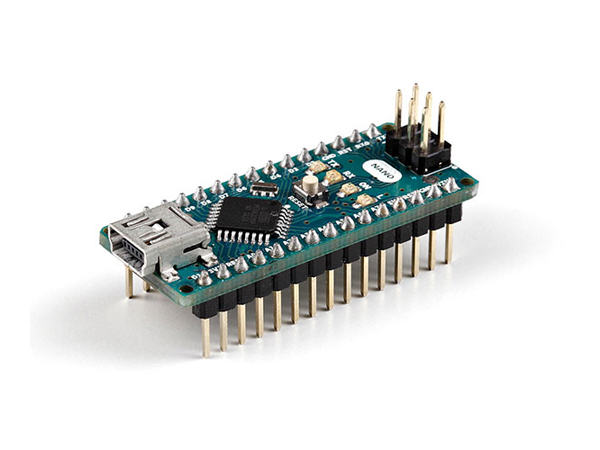
\includegraphics[width=\textwidth]{img/hardware/nano-img.jpg}
		\caption{Flower one.}
	\end{minipage}
	\hfill
	\begin{minipage}[b]{0.3\textwidth}
		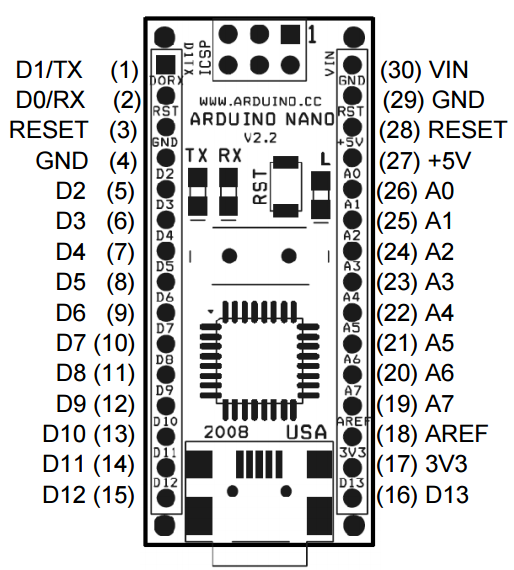
\includegraphics[width=\textwidth]{img/hardware/nano-esquema.png}
		\caption{Flower two.}
	\end{minipage}
\end{figure}




Principais características do Arduino Nano: 

\begin{itemize}
	\item Microcontrolador: É o cérebro do Arduino. Este é o dispositivo programável que roda o código que enviamos à placa. Nesta placa o microcontrolador ATmega328 é utilizado, este dispõem de 32kb de memória flash e 2kb de memória ram.
	
	\item  Conector USB: Conector que conecta o Arduino ao computador além de alimentar a placa.
	
	\item  Pinos de Entrada e Saída: Pinos que podem ser programados para agirem como entradas ou saídas fazendo com que o Arduino interaja com o meio externo.
	
	\item Pinos de Alimentação: Fornecem diversos valores de tensão que podem ser utilizados para transmitir energia elétrica aos componentes do seu projeto.
	\item  Botão de Reset: Botão que reinicia o dispositivo.
	\item  Conversor Serial-USB e LEDs TX/RX: O conversor Serial-USB permite que o microcontrolador e o computador se comuniquem, nesta placa o microcontrolador Atmega16U2 é programado para agir como conversor. Os LEDs TX e Rx acendem quando o Arduino está transmitindo e recebendo dados pela porta serial respectivamente.
	\item  Conector de Alimentação: Permite com que uma fonte alimente a placa. Caso o Arduino esteja sendo alimentado pela porta USB e por uma fonte o hardware seletor escolherá automaticamente a melhor fonte.
	\item LED de Alimentação: Indica se a placa está a transmitir energia.
	\item LED Interno: LED ligado ao pino digital 13.
	
	
	
\end{itemize}



Na tabela \ref{caraarduino} encontram-se as principais características do Arduino utilizado. 


\begin{table}[h]
	\centering
	
	\begin{tabular}{|
			>{\columncolor[HTML]{C0C0C0}}l |l|} \hline
		Microcontrolador & ATmega328 \\ \hline
		Tensão de Operação & 5V \\ \hline
		Tensão de Entrada & 7-12V \\ \hline
		Portas Digitais & 14 (6 podem ser usadas como PWM) \\ \hline
		Portas Analógicas & 8 \\ \hline
		Corrente Pinos I/O & 40mA \\ \hline
		Memória Flash & 32KB (2KB usado no bootloader) \\ \hline
		SRAM & 2KB \\ \hline
		EEPROM & 1KB \\ \hline
		Velocidade do Clock & 16MHz \\ \hline
		Dimensões & 45 x 18mm \\ \hline
	\end{tabular}
	\caption{Características do sensor TTC 104}
	\label{caraarduino}
\end{table}


O que pode ser feito? 
Evolução... 

Componentes
IDE





https://www.arduino.cc/en/uploads/Main/ArduinoNanoManual23.pdf




\newpage

\subsection{Raspberry pi }


\begin{figure}[h]
	\centering
	\begin{minipage}[b]{0.4\textwidth}
		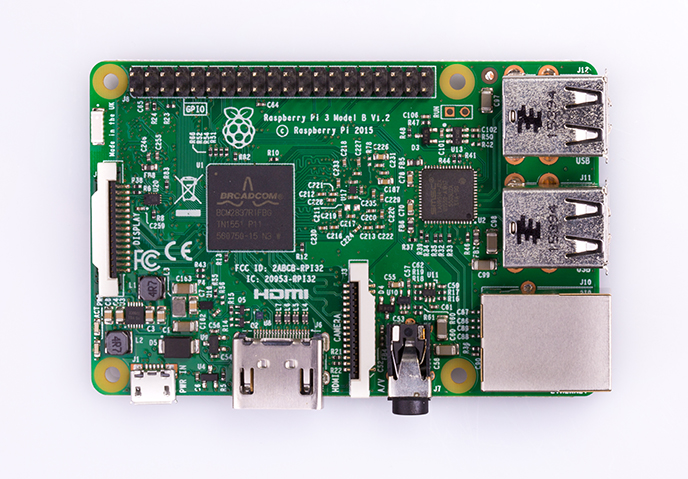
\includegraphics[width=\textwidth]{img/hardware/rasp3-img.jpg}
		\caption{Flower one.}
	\end{minipage}
	\hfill
	\begin{minipage}[b]{0.4\textwidth}
		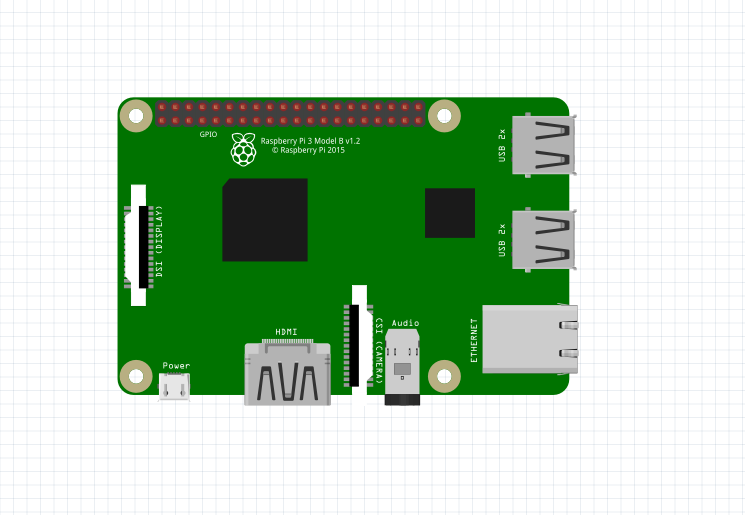
\includegraphics[width=\textwidth]{img/hardware/rasp-esquema.PNG}
		\caption{Flower two.}
	\end{minipage}
\end{figure}




\begin{table}[h]
	\centering

	\begin{tabular}{|
			>{\columncolor[HTML]{C0C0C0}}l |l|l|}
		\hline
		& \cellcolor[HTML]{C0C0C0}\textbf{Raspberry Pi 3 Model B} & \cellcolor[HTML]{C0C0C0}\textbf{Raspberry Pi 2 Model B 1.2} \\ \hline
		\textbf{Processor Chipset} & \begin{tabular}[c]{@{}l@{}}Broadcom BCM2837\\ 64Bit  Quad Core \\ Processor powered \\ Single Board Computer\\ running at 1.2GHz\end{tabular} & \begin{tabular}[c]{@{}l@{}}Broadcom BCM2837 64Bit \\ Quad Core Processor \\ powered Single Board \\ Computer running at \\ 900MHz\end{tabular} \\ \hline
		\textbf{Processor Speed} & QUAD Core @1.2 GHz & QUAD Core @900 MHz \\ \hline
		\textbf{RAM} & 1GB SDRAM @ 400 MHz & 1GB SDRAM @ 400 MHz \\ \hline
		\textbf{Storage} & MicroSD & MicroSD \\ \hline
		\textbf{USB 2.0} & 4x USB Ports & 4x USB Ports \\ \hline
		\textbf{\begin{tabular}[c]{@{}l@{}}Max Power \\ Draw/voltage\end{tabular}} & 2.5A @ 5V & 1.8A @ 5V \\ \hline
		\textbf{GPIO} & 40 pin & 40 pin \\ \hline
		\textbf{Ethernet Port} & Yes & Yes \\ \hline
		\textbf{WiFi} & Built in & No \\ \hline
		\textbf{Bluetooth LE} & Built in & No \\ \hline
	\end{tabular}
	\caption{Comparação entre versão 2 e 3 do Raspberry Pi}
	\label{my-label}
\end{table}







\newpage
\section{Sensores}

Nesta secção serão apresentados os sensores utilizados na simulação e as suas principais características. Todos os sensores foram escolhidos tendo em conta o seu enquadramento no projeto e a sua disponibilidade no laboratório. 


\subsection{Temperatura}

Como sensor de temperatura foi utilizado um termístor do tipo \ac{NTC}. Como vimo anteriormente, um termístor é um semicondutor sensível à temperatura i.e. cujo o coeficiente de variação da resistência com a temperatura é negativa, ou seja, quando a temperatura sobe então consequentemente a resistência diminui. 

Na figura x encontra-se o esquema eletrónico deste componente. 

\begin{figure}[h]
	\centering
	\begin{minipage}[b]{0.4\textwidth}
		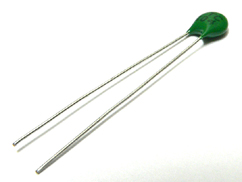
\includegraphics[width=\textwidth]{img/hardware/temperatura.jpg}
		\caption{Flower one.}
	\end{minipage}
	\hfill
	\begin{minipage}[b]{0.4\textwidth}
		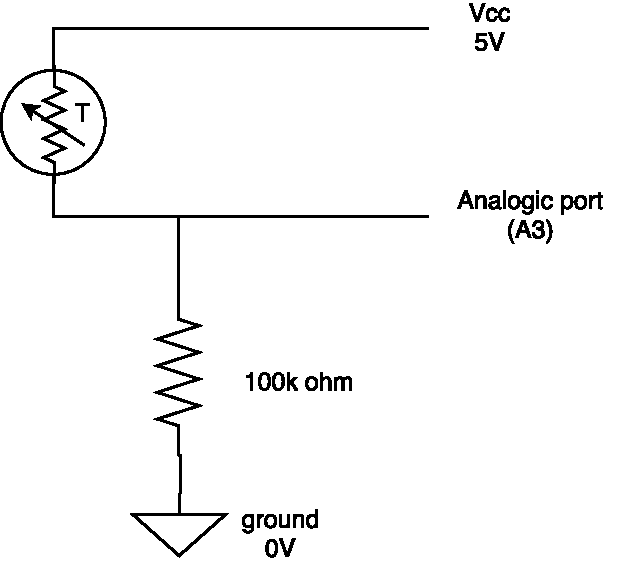
\includegraphics[width=\textwidth]{img/hardware/temp-esquema.pdf}
		\caption{Flower two.}
	\end{minipage}
\end{figure}



\begin{table}[h]
	\centering
	
	\begin{tabular}{|
			>{\columncolor[HTML]{C0C0C0}}l |l|} \hline
		Dimensão & 5mm \\ \hline
		Resistência & 100K $\Omega$  \\ \hline
		Valor máximo & +125C \\ \hline
		Valor mínimo & -30C \\ \hline
		Nível de confiança & + - 10\% \\ \hline
		Preço & 0.35 \euro/unidade \\
	\end{tabular}
	\caption{Características do sensor TTC 104}
	\label{my-label}
\end{table}



\newpage

\subsection{Luminosidade}

\begin{figure}[h]
	\centering
	\begin{minipage}[b]{0.4\textwidth}
		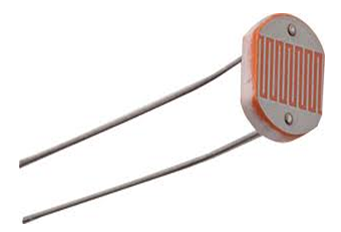
\includegraphics[width=\textwidth]{img/hardware/luminosidade.png}
		\caption{Flower one.}
	\end{minipage}
	\hfill
	\begin{minipage}[b]{0.4\textwidth}
		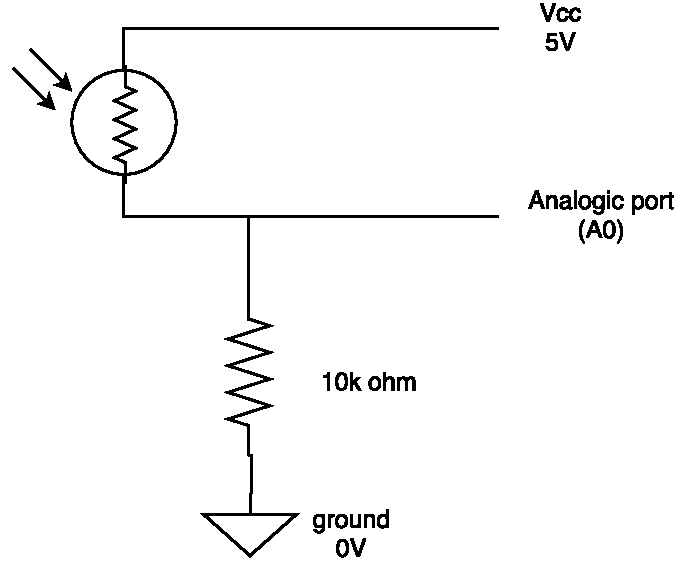
\includegraphics[width=\textwidth]{img/hardware/lumi_esquema.pdf}
		\caption{Esquema eletrotécnico}
	\end{minipage}
\end{figure}











\begin{table}[h]
	\centering
	
	\begin{tabular}{|
			>{\columncolor[HTML]{C0C0C0}}l |l|} \hline
		Diâmetro & 5mm \\ \hline
		Tensão máxima & 150VDC \\ \hline
		Potência máxima:& 100mW \\ \hline
		Tensão de operação: & -30 C a 70 C \\ \hline
		Espectro: &540nm \\ \hline
		Comprimento com terminais:& 32mm \\ \hline
		Resistência no escuro: &1 M (Lux 0) \\ \hline
		Resistência na luz: &10-20 Komega (Lux 10) \\ \hline
	\end{tabular}
	\caption{Características do sensor GL5528}
	\label{my-label}
\end{table}


\newpage
\subsection{Sensor de nível líquido}


Water Level Switch Liquid Level Sensor Plastic Ball Float


\begin{figure}[h]
	\centering
	\begin{minipage}[b]{0.4\textwidth}
		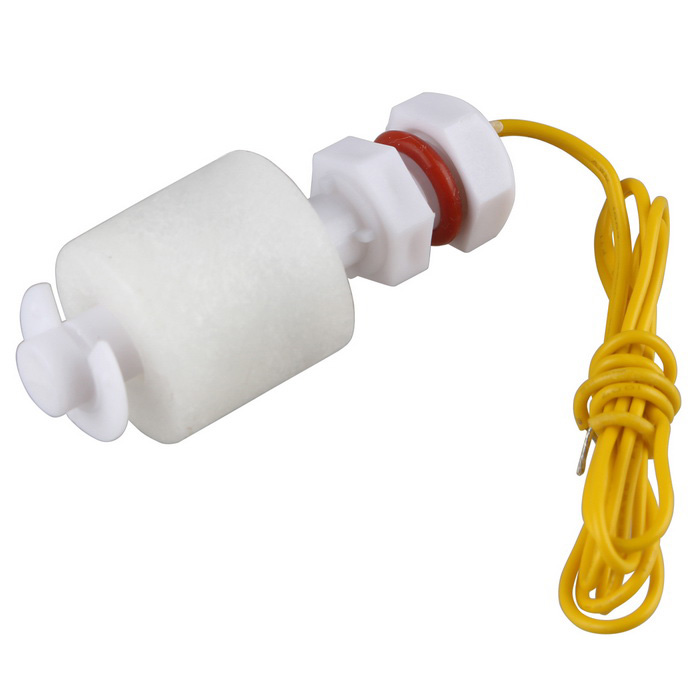
\includegraphics[width=\textwidth]{img/hardware/liquido.JPG}
		\caption{Flower one.}
	\end{minipage}
	\hfill
	\begin{minipage}[b]{0.4\textwidth}
		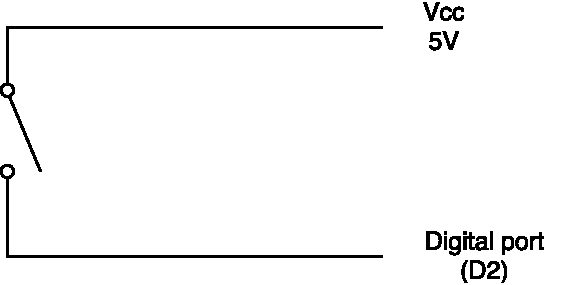
\includegraphics[width=\textwidth]{img/hardware/sw_esquema.pdf}
		\caption{Flower two.}
	\end{minipage}
\end{figure}




\subsection{Simulador de bomba para transferências de águas (led)}


dsadsa

\begin{figure}[h]
	\centering
	\begin{minipage}[b]{0.4\textwidth}
		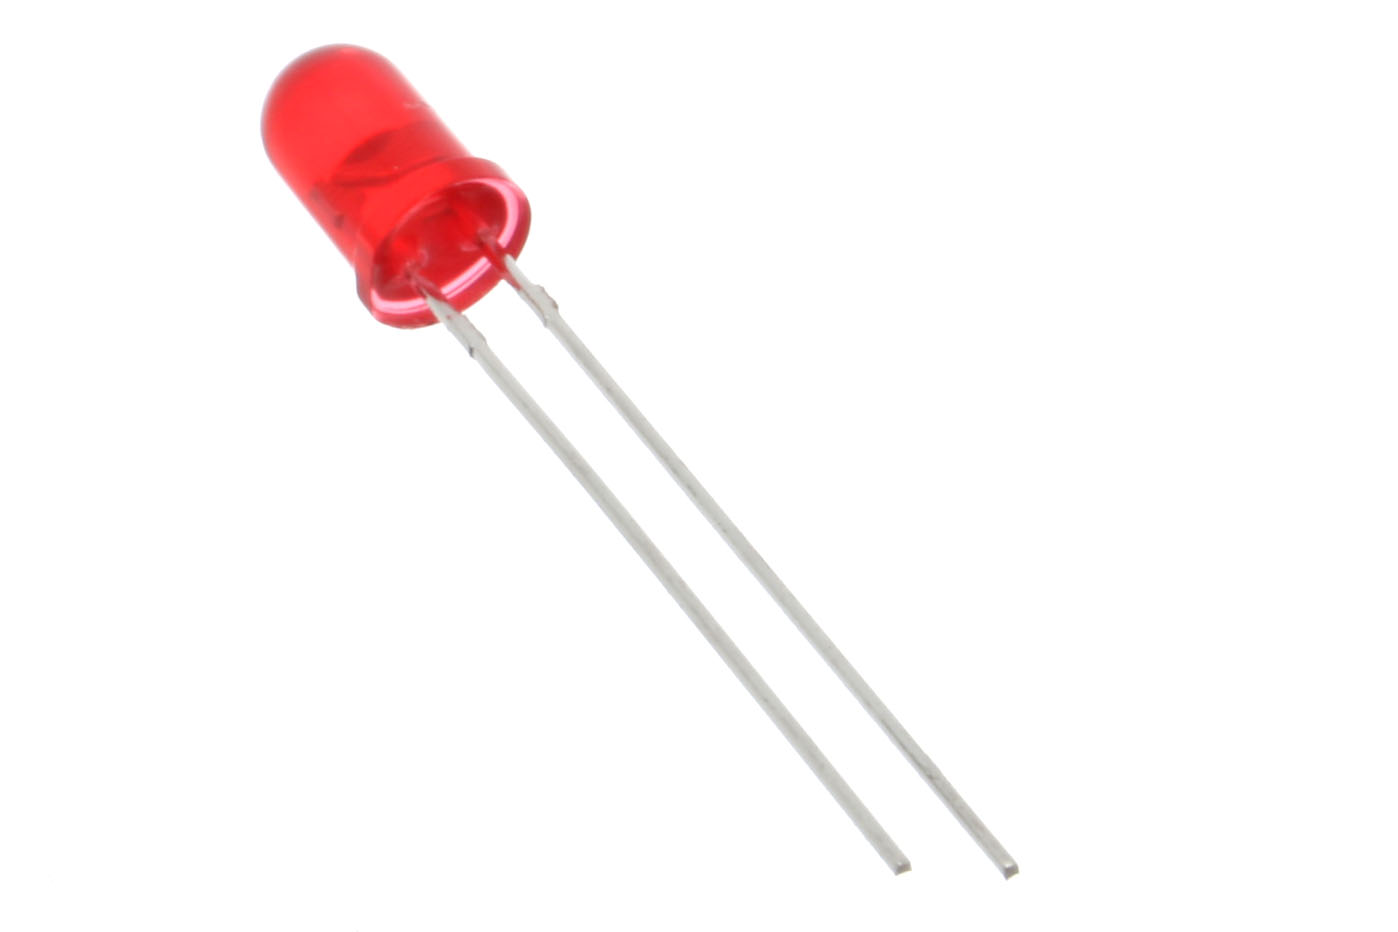
\includegraphics[width=\textwidth]{img/hardware/led.jpg}
		\caption{Flower one.}
	\end{minipage}
	\hfill
	\begin{minipage}[b]{0.4\textwidth}
		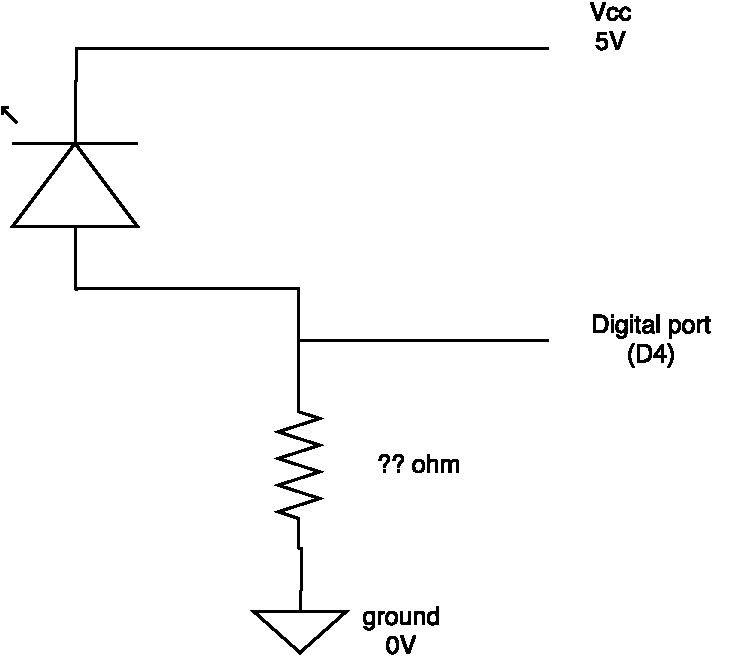
\includegraphics[width=\textwidth]{img/hardware/led_esquema.pdf}
		\caption{Flower two.}
	\end{minipage}
\end{figure}




\newpage
\section{Comunicação}



\begin{figure}[!htb]
	\centering
	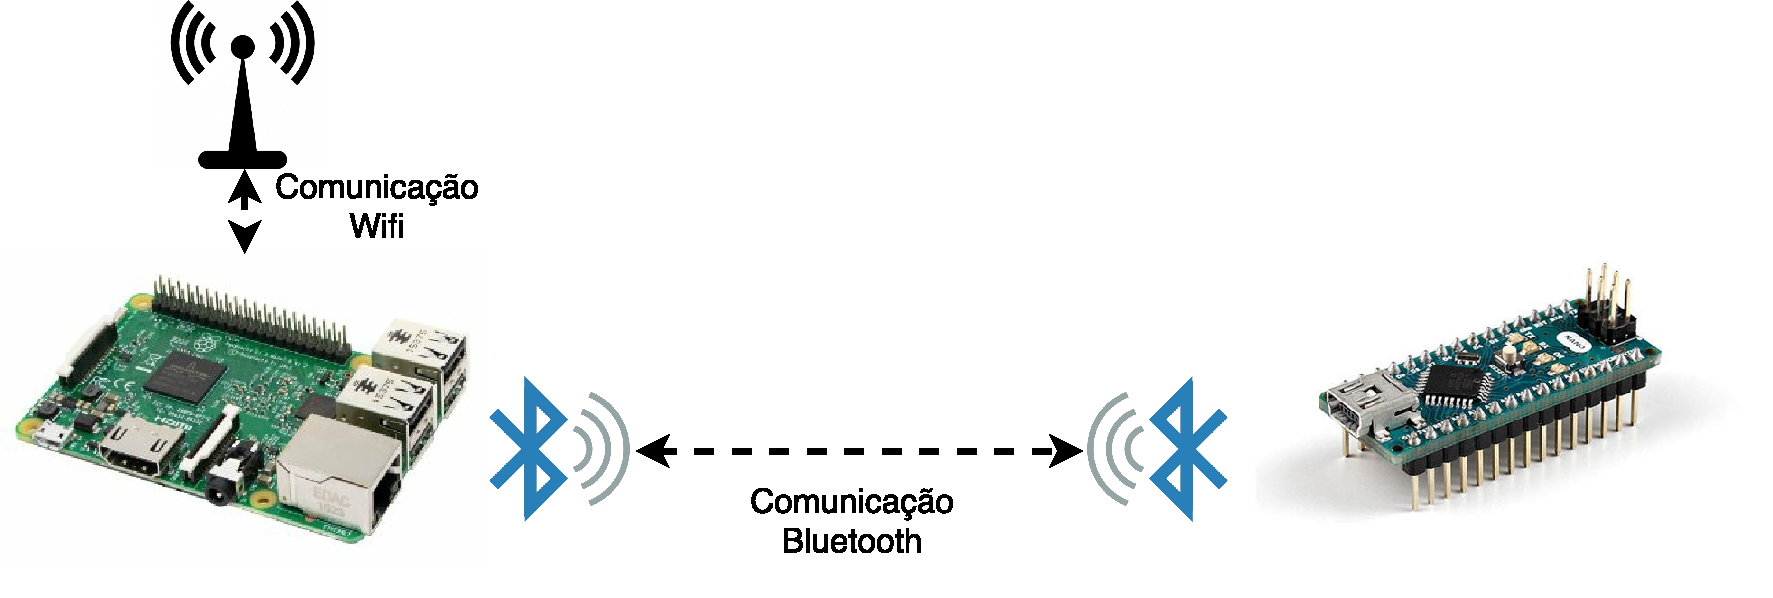
\includegraphics[width=\linewidth]{img/comm-blue/HW-geral.pdf}
	\caption{Arquitetura lógica}
	\label{opencvlogo}
\end{figure}




Numa primeira fase precedeu-se à comunicação através de porta serie. 





\begin{figure}[h]
	\centering
	\begin{minipage}[b]{0.4\textwidth}
		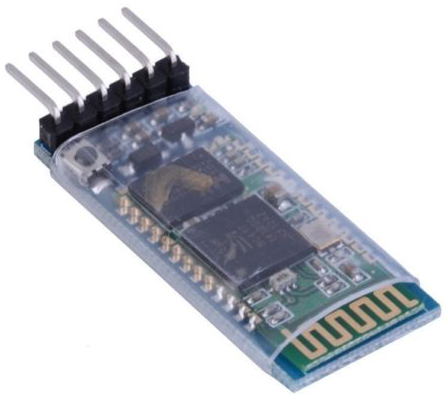
\includegraphics[width=\textwidth]{img/hardware/bluetooth_zs-040.png}
		\caption{Flower one.}
	\end{minipage}
	\hfill
	\begin{minipage}[b]{0.4\textwidth}
		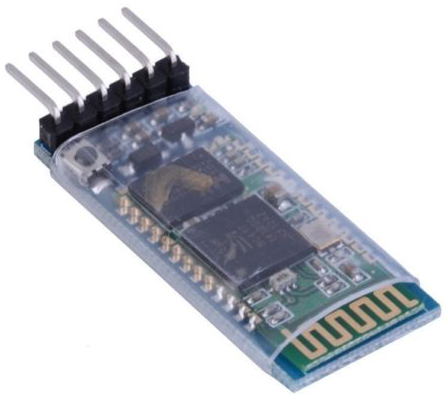
\includegraphics[width=\textwidth]{img/hardware/bluetooth_zs-040.png}
		\caption{Flower two.}
	\end{minipage}
\end{figure}


http://www.instructables.com/id/Modifying-the-AT-Codes-on-a-HC-05-With-the-Code-ZS/


http://www.arduinoecia.com.br/2013/03/modulo-bluetooth-jy-mcu-configuracao.html


Testar ligação com modulo foi usada app bluetooth Terminal HC-05






\newpage
\section{Interligação de componentes}





\section{Considerações finais}


>1 fase testar coneccao arduino to rasp via porta serie; foi criado um script em python para processar info e enviar para o servidor através da API 

>2 fase : necessidade de tornar um módulo isolado sem necessidade de fio; foi testado um modulo wifi e bluetooth; 

>neste contexto modulo wifi nao!... pretende-se que os sensor moduels sejam de baixo custo e low power. foi utilizado um modulo bluetooth; foi testada a conexao da comm bluetooth através de uma client disponveil na google play bluetooth terminal HC-05 


> 
pq nao foi usado um sensor de salinidade?



 

